Next we discuss each of the replications in more detail and highlight the substantive insights that can be drawn from the AME framework.

\subsection{Re-estimation of Reiter \& Stam (2003)}

\citet{reiter:stam:2003} examine the relationship between democracy, dictatorship and the initiation of militarized disputes. Their work contests prior scholarship that had claimed interstate dyads containing democracies and personalist dictatorships were particularly prone to conflict because of aggression on the part of the democratic state. Using directed dyads, they find evidence against this hypothesis: dictators are in fact more likely to challenge democracies, but not the other way around.  In addition, military regimes and single-party regimes are more prone to initiate disputes with democracies, but the opposite is not true. Independent variables focus on various encodings of regime types, contiguity, alliance, and capability measures. As is prevalent in this literature, Reiter \& Stam employ a logistic regression that includes an indicator of the time since the last dispute as well as three cubic splines. The database for this study is constructed using \texttt{EUGene} \citep{bennett:stam:2000} and comprises approximately three-quarters of a million stacked dyads. Based on their statistical analysis, they conclude that institutional constraints affect the propensity of democratic and non-democratic leaders to engage in military conflict. 

In the original model, the variable ``Pers/Democ Directed Dyad" (which represents a Personalist $\rightarrow$ Democractic directed dyad) has a positive effect while the variable ``Democ/Personalist Directed Dyad'' is too imprecisely measured to indicate a direction. In our re-estimation using the AME framework, we also find that Pers-Democ directed dyad has a positive effect while Democ-Pers directed dyad is still too imprecisely measured to indicate a direction. Using this model, however, we can no longer conclusively say that the Pers/Democratic coefficient is larger than the Democ/Personalist one.\footnote{Comparing } Our re-estimation using the AME approach therefore cast some doubt on Reiter \& Stam's key claim that MIDs initiated by personalist dictatorships against democracies are more likely than MIDS initiated by democracies, though many of the major effects  uncovered by the authors remains robust when accounting for dyadic interdependencies. %Further, the effect of most of the covariates in the literature thought to predict interstate MIDs are much closer to zero when using the AME framework suggesting that some of their effects were actually the products of interdependencies. 

\subsection{Re-estimation of McDonald (2004)}

\citet{mcdonald:2004} studies whether trade promotes peace between nations. \citet[p. 547]{mcdonald:2004} introduced the argument that free trade between states ``makes conflict less likely because of its efficiency over conquest in acquiring resources\ldots''. Accordingly, he provided evidence challenging the generalized linkage between peace and trade and refined the measurement of the standard ``trade'' variable, arguing that \textit{free} trade, rather than trade alone, reduces the likelihood of conflict between states. His key hypothesis is that greater levels of protection increase the probability of interstate conflict, an argument that builds on the work of classic liberalism and connects free trade to the power of domestic audiences. \citet{mcdonald:2004} measured free trade in two ways. The first, the ``protection'' variable measures the proportion of customs revenue divided by total imports in the state that possesses the greater such ratio in each dyad; this reflects the notion that larger protected sectors generate greater societal pressures resulting in pockets of support for war. This measure thus captures the score of the state in the dyad that possesses higher barriers to trade. \citet[p. 560]{mcdonald:2004} also includes a measure of economic integration  calculated as ``the lower proportion of total dyadic trade (imports plus exports) divided by state $i$'s GDP or total dyadic trade divided by state $j$'s GDP''. The (binary) dependent variable is the onset of a new militarized interstate dispute within a given dyad, and \citet{mcdonald:2004} includes splines to correct for temporal dependence with robust standard errors clustered on each dyad.

\subsection{Re-estimation of Weeks (2012)}

\citet{weeks:2012} examines the influence of domestic institutions on the initiation of military conflicts by autocratic leaders.  She argues that in some circumstances autocrats are held accountable for their foreign policy decisions. She adds the nuance that autocratic audiences are not homogeneous. When the autocratic regime is nonmilitary, domestic audiences do not favor military actions, but in military autocracies this is not the case. Further she argues that in personalistic regimes without a military or civilian domestic audience, the leaders tend to be more likely to employ military force in their foreign policy.  To study this question, she uses a dyadic design in which the dependent variable is ``whether country A in a directed dyad initiated military conflict against country B during year t'' (page 337).  One major innovation in her study resides in the nuanced way in which she conceptualizes and codes regimes into four types: a) Machine, b) Junta, c) Boss, and d) Strongmen. She also includes a variety of putative control variables focusing on capabilities for both sides of the dyad, alliances, geography, trade dependence, regime instability, and the regime type of ``side B.'' She uses a logistic regression, but follows \citet{beck:etal:1998} and includes splines to capture temporal covariation in the dependent variable along with fixed, unit effects. The analysis is done for dyads, but is considered to be from the perspective of the actor that initiated the dispute. The basic finding is that a) juntas, boss type, and strongmen type regimes are more likely to initiate conflict than machine-type regimes (and maybe democracies) and that b) machine-type regimes are no more belligerent than democracies.   These insights are mainly emphasized in the paper by the parameter estimates depicted in Tables 1 and 2 (pages 339--340) from the paper. She argued that ignoring important nuances between different types of autocracies hinders our understanding of the initiation of military conflict by autocracies. 

\begin{figure}[!h]
	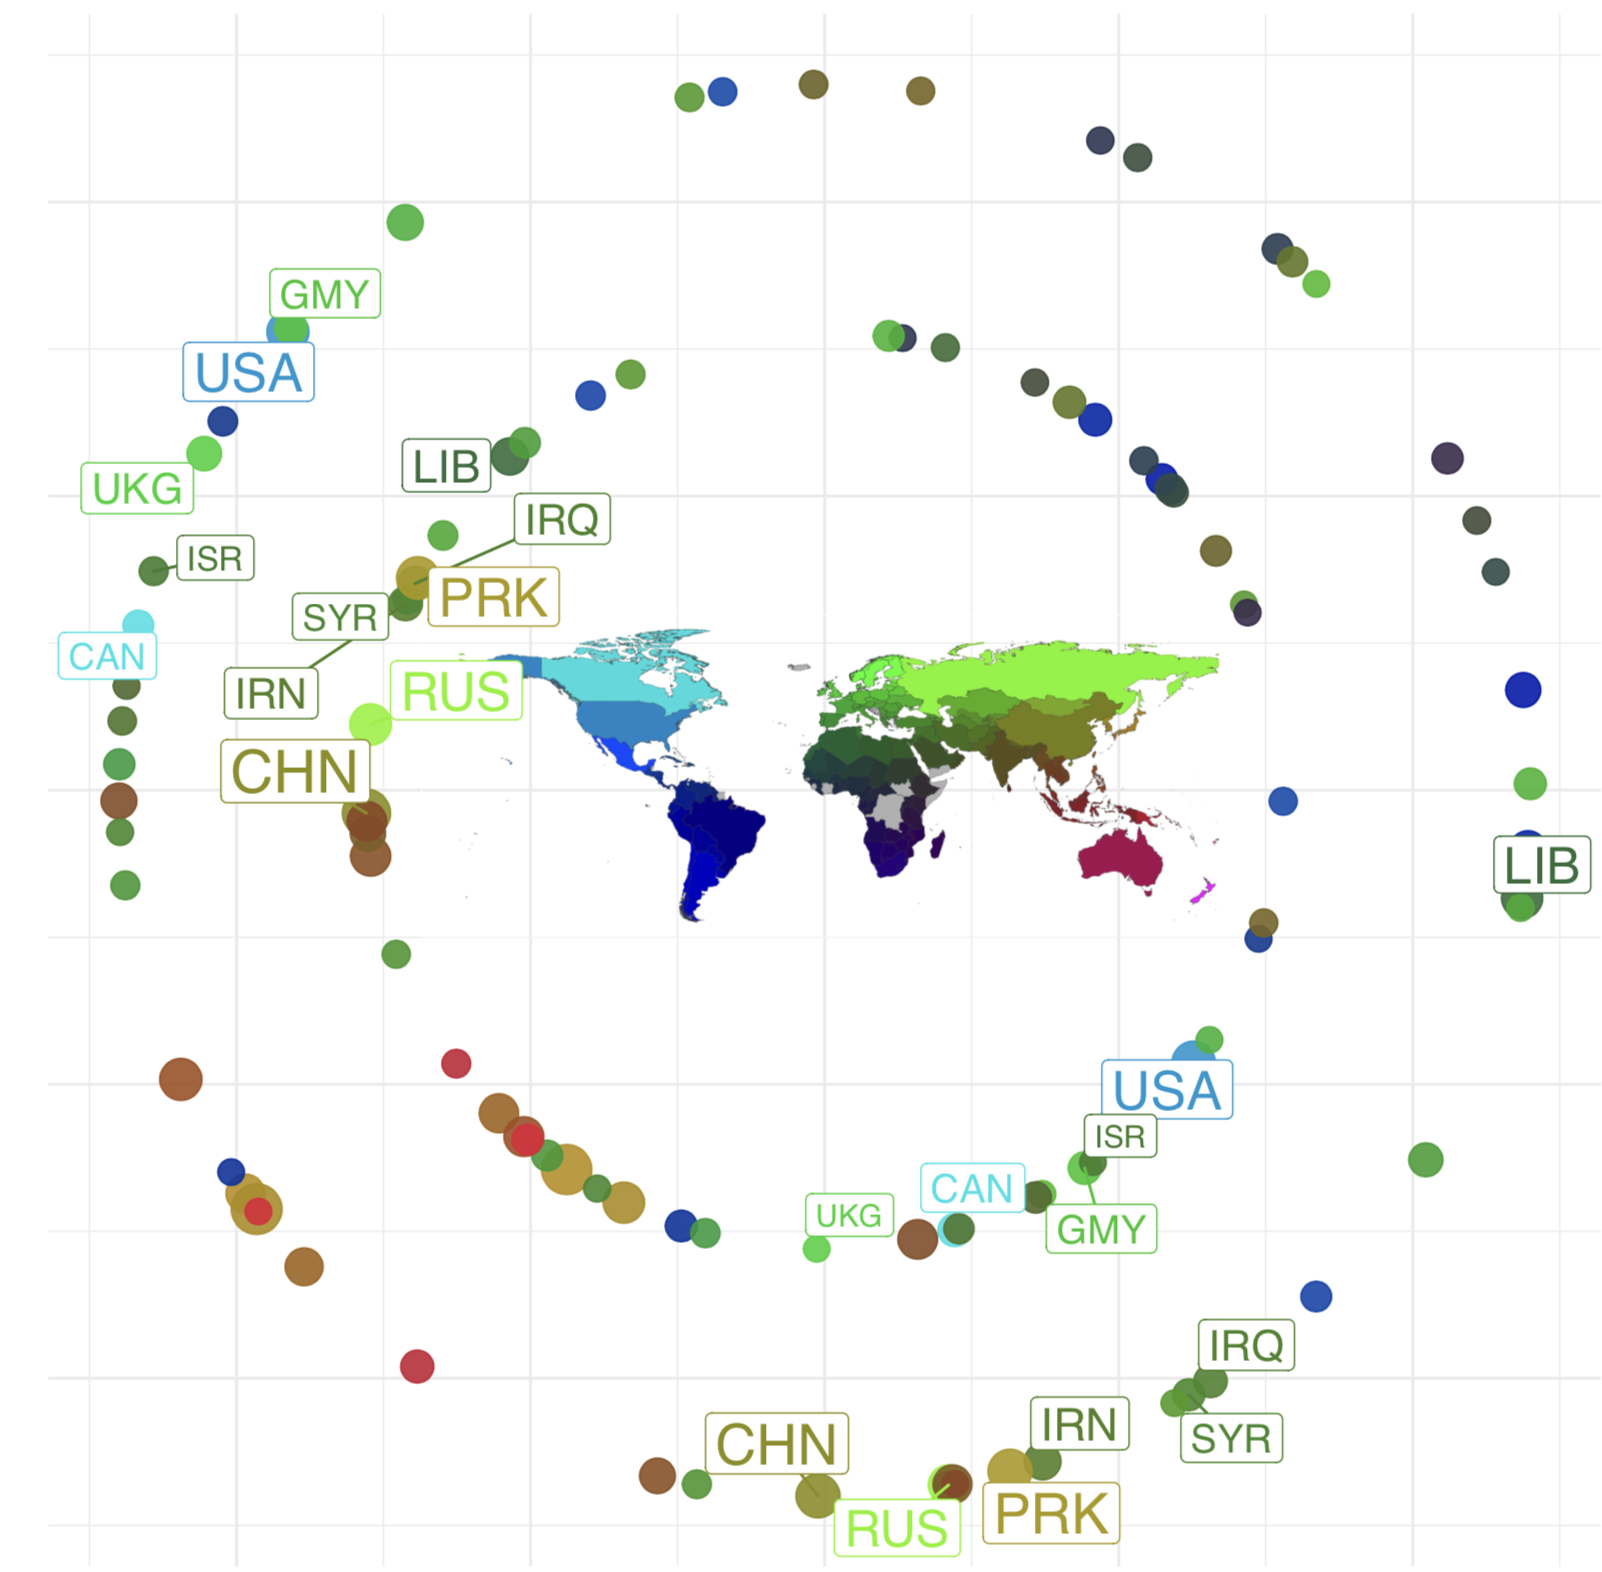
\includegraphics[width=\textwidth]{weeks_circPlot.png}
	\caption{ Visualization of multiplicative effects for Weeks (2012). Each circle designates a country and the color corresponds to the legend at the center of the visualization. Countries that cluster together in the outer ring are those that were found by the model to have similar sending patterns, meaning that they tend to send conflict to similar sets of countries. The inner ring clusters countries by the similarity of who they receive conflict from. 
	%Blue represents groups with common sending patterns and red represents groups with common receiving patterns.
	}
	\label{fig:weekscirc}
\end{figure}
\FloatBarrier

The re-estimation of \citet{weeks:2012} has the sharpest divergence between the GLM results and those of the AME Model. In Weeks' initial models,  she finds that machines are less prone to initiate conflict than the reference category, whereas Juntas, Bosses, and Strong-men are more conflict-prone. When we examine the AME results, we find that none of these values are distinguishable from zero. Similarly, we find less pronounced effects for military capabilities. One explanation for this divergence is the AME model's ability to account for third-order effects. Inspection of the multiplicative effects in Figure~\ref{fig:weekscirc} reveals a number of clusters of states which exhibit structural equivalence---in the top left corner we see the US, the UK, Germany, Canada, and Israel. These states cluster together in the outer ring of this visualization because they tend to send conflicts to similar targets. Conversely, in the bottom right of the outer ring, we see a cluster of authoritarian countries: Iraq, Russia, Syria, North Korea, and China. In the inner ring, the proximity of countries is determined by the degree to which they receive conflict from the same countries. In general, the clusters found on both the inner and outer rings have similar governmental types (Iraq, Syria, Libya, and North Korea all fell under the ``boss" category). They tend to initiative and be targets of conflict by similar actors but they are not more likely to initiate 

Thus she is kinda right but wrong in that they are more likely to intiate conflict in general ... but they do have a similar pattern of relationshsips

In the GLM, which ignores these third-order dependencies, many of these results might have been attributed to regime type. Structural equivalence is present even when accounting for nodal characteristics like regime type.  The AME model, on the other hand, shows that this can be specified in terms of the interdependencies captured by the multiplicative effects. 

\subsection{Re-estimation of Gibler (2017)}

A more recent example is \citet{gibler:2017} which examines the onset of militarized disputes using capabilities, joint democracy, alliances, and power parity in a undirected dyadic study using logistic regression and dyad clustered standard errors. In addition, Gibler shows that the long-standing relationship between the relative parity of capabilities and initiation of international conflict is almost completely mediated by the initial conditions for the members of the dyad when they joined the international system as sovereign members. This finding calls into question many IR theories about the role of balance in terms of generating international conflict \citep{organski:1958}.

We re-estimated model 6 from Table 6 (2017, 34). The results are presented in the Appendix. The results obtained with AME stand in stark contrast to those found with a logistic regression (with dyad clustered, robust standard errors).  Most importantly, the primary variable from the Gibler study, parity of the members of a dyad at the year in which they entered the international system, is shown to be unimportant in the AME results.  Not only is the value of this parameter small, but it has a very large relative standard error---over a magnitude larger than the parameter itself ($z= 0.038$). In addition, the variable indicating whether both members of the dyad were coded as democracies (joint democracy) follows the same pattern: important and strong in the logistic results, but this disappears once interdependencies are modeled.  As might be expected, the strong geographic clustering in the original study is about one-quarter as strong in the AME estimations. Similarly, rivalry coefficients are about one-third the size in the AME formulation, but a great deal more precisely measured ($z=18.116$). 

\begin{figure}
	\caption{Marginal effects of a change in the Rivalry variable for both the AME and the Gibler estimation.  \label{fig:gibmargeff}}
	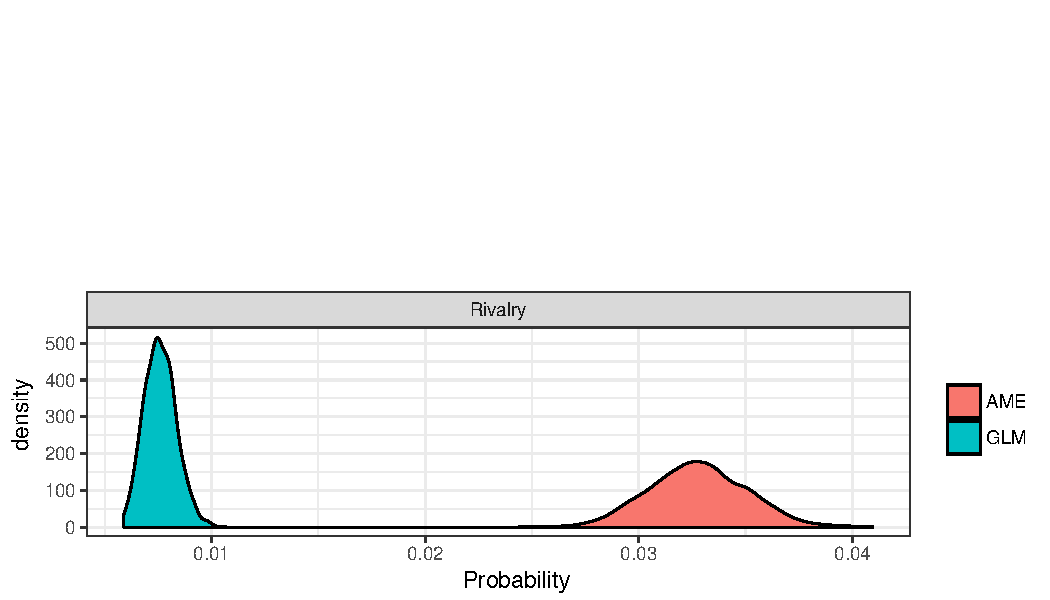
\includegraphics[width=\textwidth]{gibler_margeff.pdf}
 	\label{fig:gibmargeff}
 \end{figure}

We utilized the original and the AME results from Gibler's model 6 in Table 6 to calculate the expected values for one scenario focusing on the variables measuring rivalry.  We employed mean or modal values for all independent variables, except we changed the rivalry variable to indicate that there was a rivalry when the actual data suggest there is none.  The expected values of this scenario are essentially a first difference plot comparing results with the model when estimated in two different ways: Gibler's GLM estimation and our AME approach.  As this Figure~\ref{fig:gibmargeff} illustrates, the AME results differ notably. First, the expected value of the dependent variable---the probability of the onset of a militarized interstate dispute, is considerably lower when taking interdependencies into account with the AME model.  These are rare events, so the probabilities are low, but the difference is a factor of almost 2. Thus, you get quite substantially different expected values from these two models.  

\subsection{Lessons Learned from Re-estimating Five Prominent Studies}

First and foremost, many findings that emerge from models that do not take interdependencies into account lose their statistical significance when network effects are estimated via AME. Not only are coefficients biased in the GLM approaches to the analysis of dyadic data, but they are often imprecisely measured, with poorly calibrated standard errors.  This means that significance testing (for better or worse) is compromised when network effects are ignored.

Second, even when the results from the AME estimation conform with those found in an OLS or logistic regression, new insights emerge from the additional information derived. In particular, there is actual information about the dependencies so that clusters can be identified, and the extent of reciprocity at the dyad level, as well as among senders and receivers.  This kind of information is absent in standard approaches and adds to our ability to explain specific as well as general results.

Third, it is evident that the actual results---not the estimated coefficients and their covariances---which are generated by the models differ greatly in expectations.  This implies that policy experimentations with the models, as well as scenario-based simulations and forecasting of GLM models are likely to often give misleading results compared to the AME approach.

Fourth, it is clear that the AME approach dominates the GLM approaches in terms of performance. Not only it is better at correctly identifying cases in which the dependent variable takes a value of $0$ (via the ROC curves and associated statistics), but it also dominates at correctly identifying occurrences of the dependent variable in the data (seen via the PR curves and associated statistics). In the case of the study with a continuous dependent variable, the AME approach has average error statistics that are about one-half that found in the original model. 